% Chapter 1


\chapter{old Introduction} % Main chapter title

\label{Chapter1} % For referencing the chapter elsewhere, use \ref{Chapter1} 
The idea of \textbf{reinforcement learning} has been known since \textbf{Turing}'s time.
He talked about it in his article "Computing machinery and intelligence \cite{turing2009computing}":
"We normally associate punishments and rewards with the teaching process. 
Some simple child machines can be constructed or programmed on this sort of principle. 
The machine has to be so constructed that events that shortly preceded the occurrence of a punishment signal are unlikely to be repeated. In contrast, a reward signal increased the probability of repetition of the events, which led up to it." 
From that time to our day, a lot of progress is being achieved.\\

The first one was \cite{tesauro1995temporal} TD-Gammon in 1995.
An artificial neural network develops by Gerald Tesauro for IBM trained with an RL algorithm called TD-Lamba.
It was able to play backgammon, almost like a high-level human player.

\begin{figure}[h]
\centering
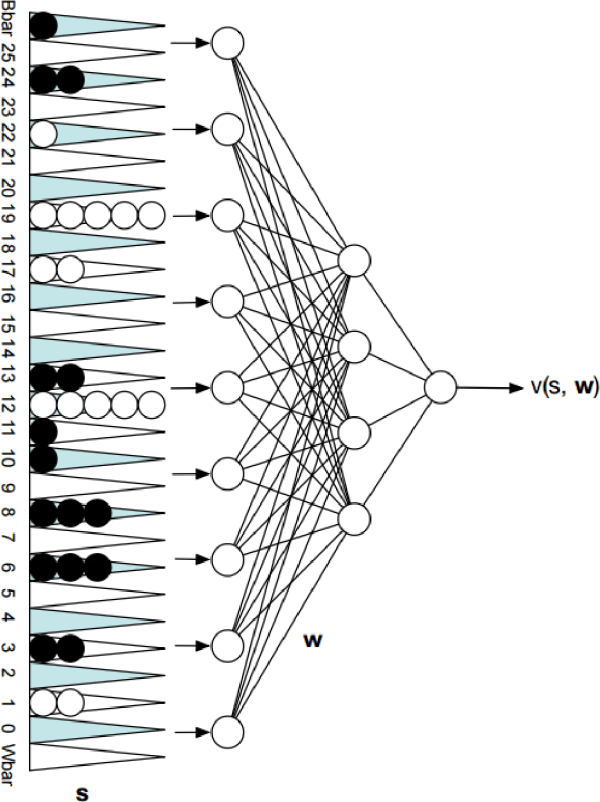
\includegraphics[width=.6\textwidth, height=.5\textheight]{pictures/td_gammon}
                  \caption{ Illustration of TD Gammon’s Neural Network.}
            \end{figure}

For the second big event in the reinforcement community, we have to wait until 2015. 
In particular, we have to wait for the Deep Learning era.
In 2015 the Deep Q-Network algorithm was developed by DeepMind \cite{mnih2015human}. 
It solved many Atari 2600 games from the Arcade Learning Environment, directly from high-dimensional sensory input and no architecture or learning algorithm adjustment. 

\begin{figure}[H]
\centering
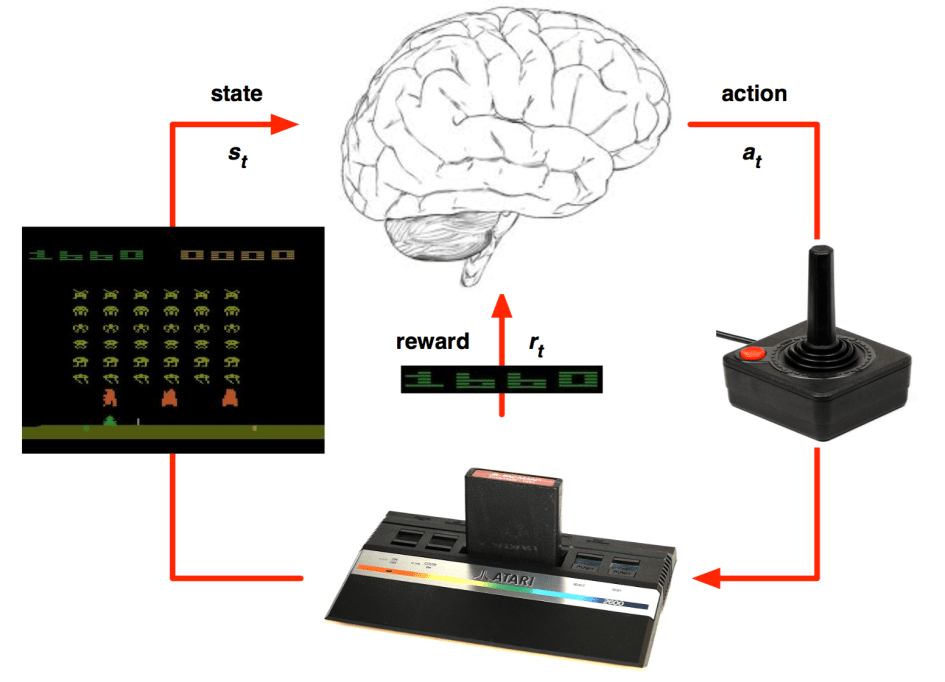
\includegraphics[width=.6\textwidth, height=.3\textheight]{pictures/dqn_intro}
                  \caption{ Structure of DQN applied to Atari Games.}
            \end{figure}

In 2016 DeepMind released Alpha Go \cite{silver2016mastering}: the first IA capable of beating the board game's human champion called Go for the first time in history.
Go was never mastered before because of the prohibitively set of possible moves useless for the heuristic search and the alpha-beta pruning methods.
To have an idea, for the game of chess, the number of all possible moves at each step is 35 for a total of $10^{123}$ possible moves.
In Go, this number is 250 for a total of $10^{360}$ possible moves. 

\begin{figure}[H]
\centering
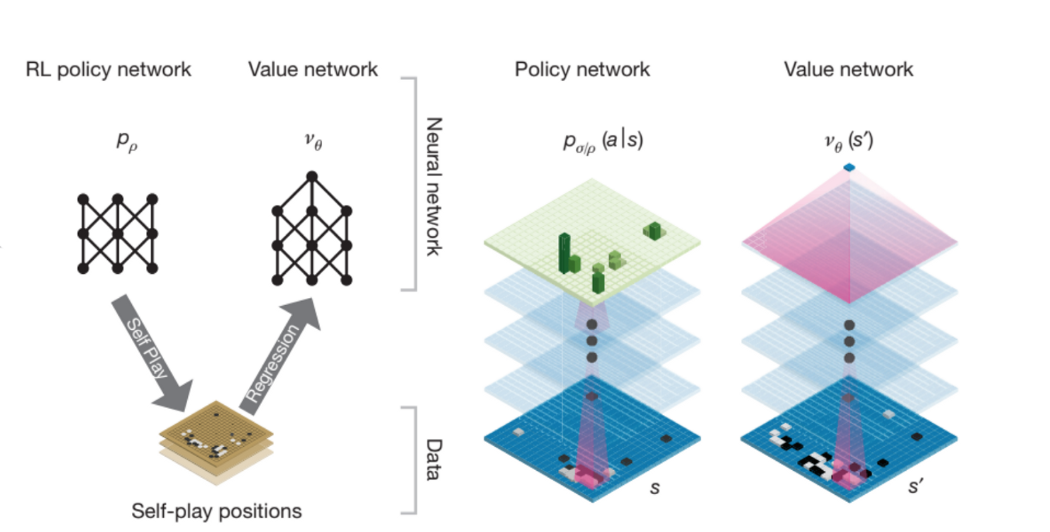
\includegraphics[width=1.\textwidth, height=.3\textheight]{pictures/alpha_go}
\caption{ Neural networks schema from Alpha Go .}
            \end{figure}

Lastly, in 2018 OpenAI \cite{andrychowicz2020learning} trained a human-like robot hand to manipulate physical objects with unprecedented dexterity. 
The task consisted of placing a cube in the robot hand and ask the agent to move it in a different orientation.
A typical task example could be asking the agent to rotate the block to put a new face on top. The network observes only the coordinates of the fingertips and the images from three regular RGB cameras.
Since this kind of training requires much experience, the training interactions are computed in a simulator, and then the trained policy is transferred to the physical robot.

\begin{figure}[H]
\centering
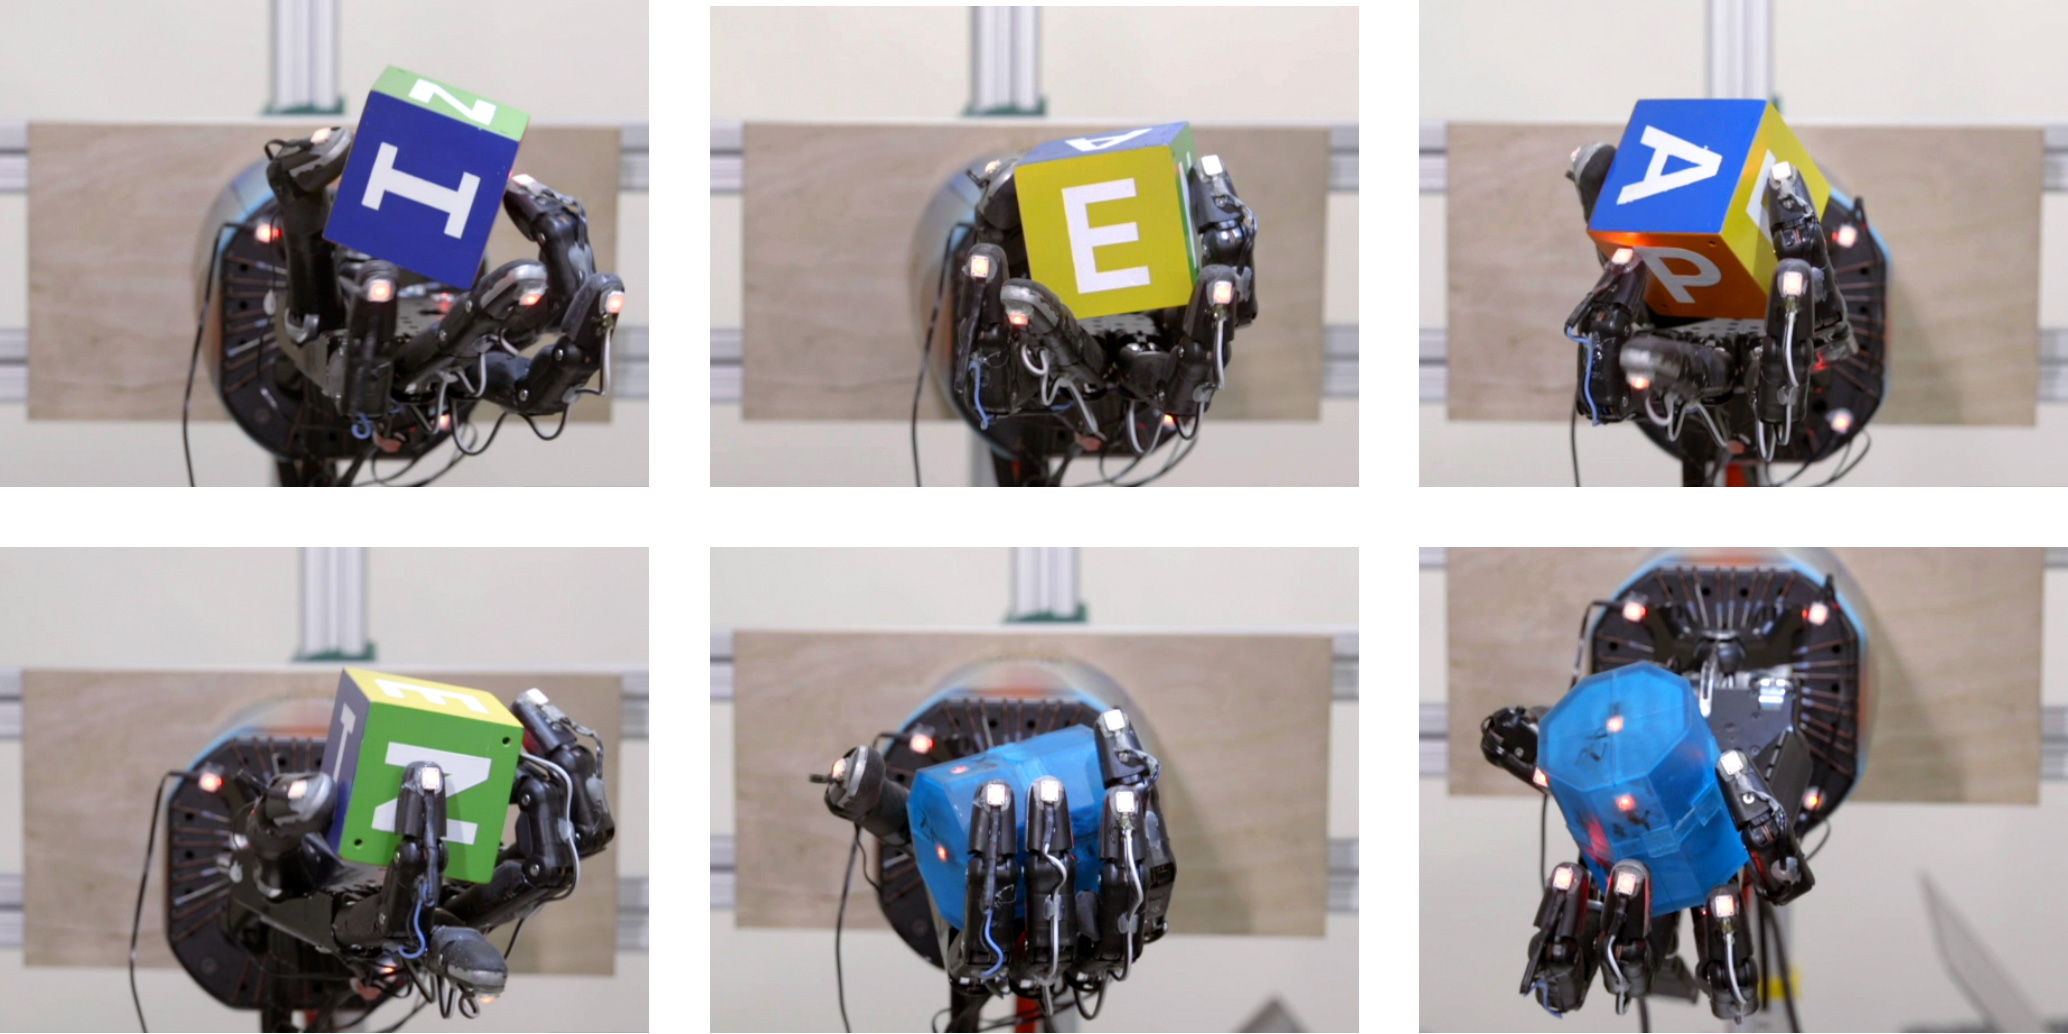
\includegraphics[width=1.\textwidth, height=.3\textheight]{pictures/robot_hand}
\caption{ Open AI agent manipulates the different type of objects in the real world.}
            \end{figure}
            

Despite all this successful story, the reinforcement learning problem is not solved, and it is still not possible to train agents in the real word for challenging tasks.

In 2019 Open AI released Open AI Five: the first AI able to beat the world champions in an e-sports game called Dota 2. 
Despite the incredible result, the training cost was tremendous.
"In total, the current version of OpenAI Five has consumed 800 petaflops/s-days and experienced about 45,000 years of Dota self-play over 10 real time months, for an average of 250 years of simulated experience per day."

In all the works cited below, the agent was trained in a simulator, in which it is possible to accumulate many interactions in short periods.
For example, the human-like robot hand required years of simulated experience, 3 for a simple case, and 100 to make the policy robust to different physical dynamics.

\begin{figure}[H]
\centering
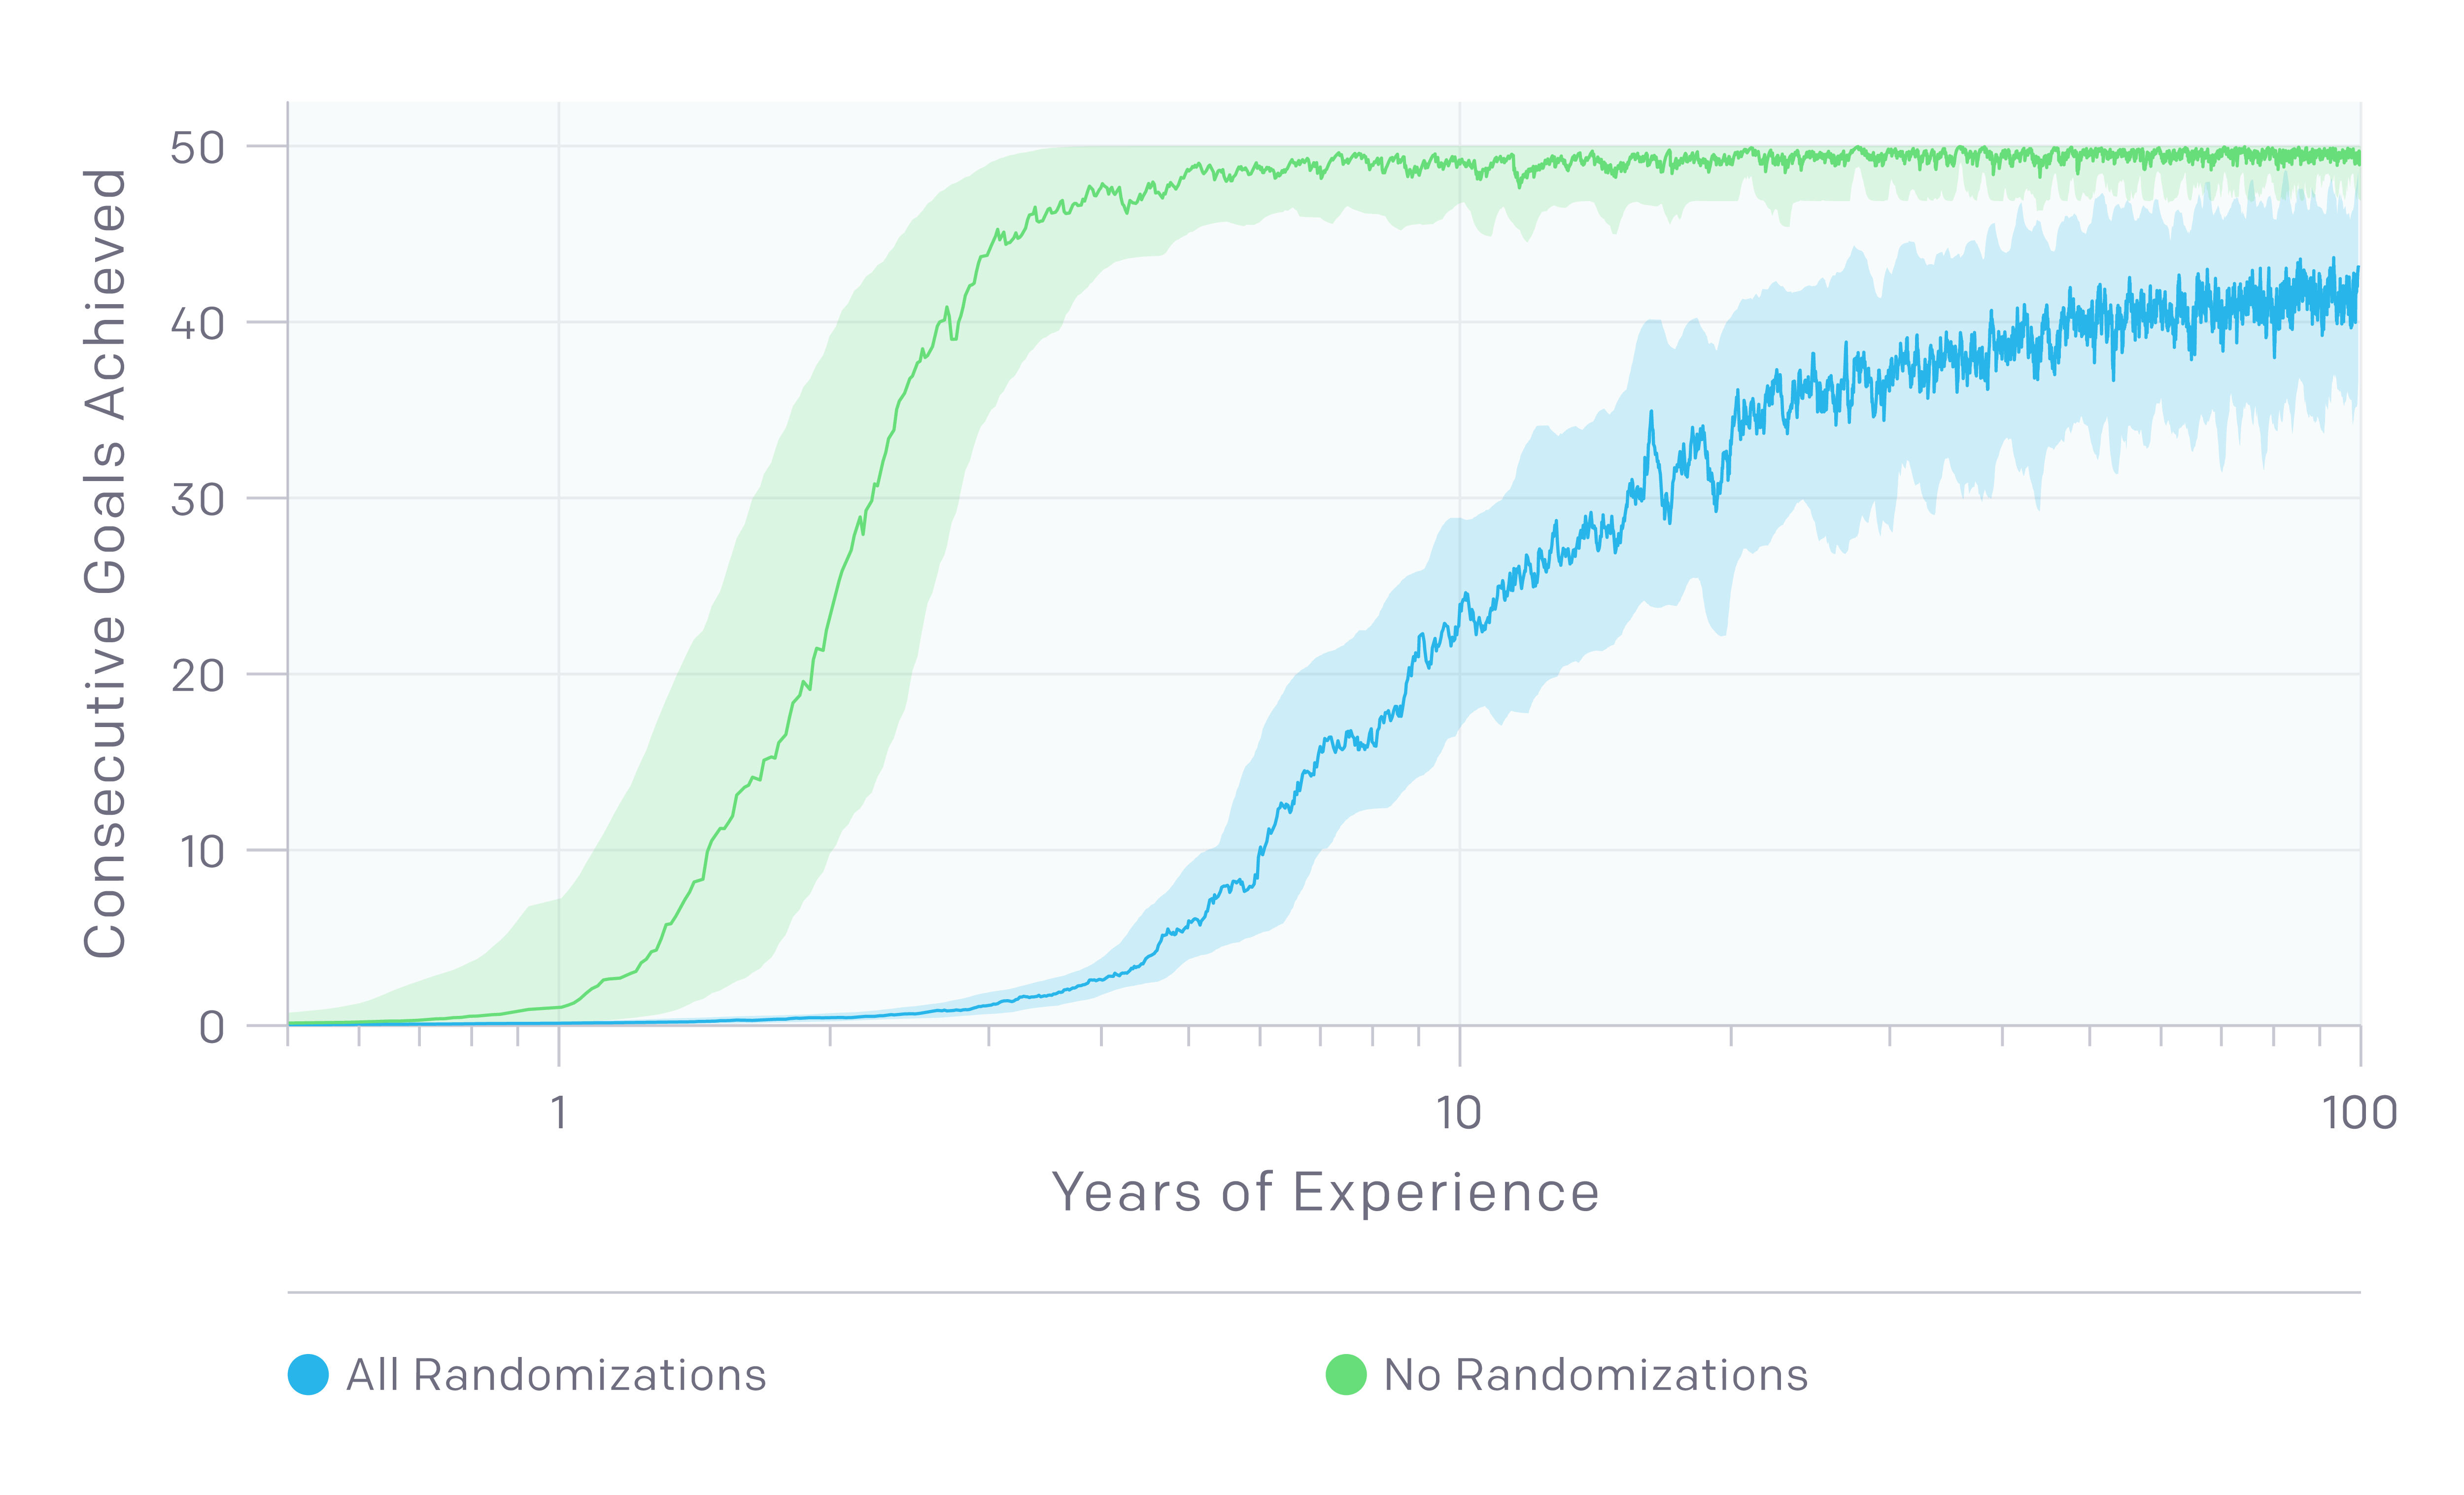
\includegraphics[width=1.\textwidth, height=.3\textheight]{pictures/years_robot_hand}
\caption{ Learning progress with and without randomizations over years of simulated experience.}
            \end{figure}

Collect real-world sample is very expensive, so it is practically impossible to use those algorithm outside of the simulator.
Is it possible to reach a similar performance without this massive amount of data?

Alan Turing had already foreseen this problem, and in his article, he says: "The use of punishments and rewards can at best be a part of the teaching process... By the time a child has learned to repeat 'Casabianca' he would probably feel very sore indeed".

One of the most promising solutions is the Model-Based approach that combines the power of supervised learning, the reinforcement learning framework, and the planning algorithms.

In this thesis, we want to find out how much this approach can really improve the performance of the model-free algorithms. To understand that one of the state-of-the-art Model-Based DRL algorithms called PlaNet is deeply investigated and compared with the model-free DRL algorithm called Deep Deterministic Policy Gradient (DDPG).
All the experiments are based on Deepmind Control Suite that is a set of continuous control tasks that are built for benchmarking reinforcement learning agents.  The main strengths and weaknesses of both approaches are highlighted and in addition to that, some ideas for the improvement of PlaNet will be tested.





